%% This is an example first chapter.  You should put chapter/appendix that you
%% write into a separate file, and add a line \include{yourfilename} to
%% main.tex, where `yourfilename.tex' is the name of the chapter/appendix file.
%% You can process specific files by typing their names in at the 
%% \files=
%% prompt when you run the file main.tex through LaTeX.
\chapter{Introduction}

Finding a practically shortest route on a large road network in a metropolis is not only of algorithmic interests, but also of economic and environmental values. Less travelling time means less fuel consumptions and less carbon emissions. However, finding shortest routes can be challenging, especially when the road traffic is known to be \emph{time-dependent} or \emph{dynamic}, namely, the road conditions change with time. It may take 10 minutes on average to travel through a particular road at 10a.m, but it is possible that the expected travel time increases to 20 minutes at 5p.m. Moreover, two different roads may have different time-varying patterns. For instance, one road may have a peak traveling time at 12p.m but the other may have two peaks at 8a.m and 6p.m, respectively.

The general time-dependent shortest path problem can be formally defined as follows.
\begin{defn}
In a weighted, directed graph $G=(V,E)$ representing a road network with a weight function $w : E,t \rightarrow \mathbb{R}$, given an origin $u$, a destination $v$ and a departure time $t$ from $u$, find a path $P$ that satisfies:
\begin{equation}
\delta_P(u,v)\leq
\end{equation}
\end{defn}

A typical Bellman-Ford\cite{CLRS09} or Dijkstra's algorithm\cite{Dij59} for finding shortest paths assume the cost of traversing each edge in an abstract graph is constant with respect to time and therefore, do not work on time-de\-pendent road networks without appropriate modifications. Fortunately, most online mapping services such as Google Maps or Apple Maps are able to recommend shortest routes by incorporating real-time traffic information. This project seeks to investigate yet another alternative approach of finding shortest routes on a large road network, which is based on mining a GPS\footnote{Global Positioning System} trajectory database aggregated from thousands of taxies in Beijing, China.

Chapter two defines several important concepts used in this project. 

Chapter three gives an overview of the GPS-based approach.

Chapter four describes the data pre-processing and presents a novel neural network-based outliner detection method.

Chapter five elaborates the process of building a landmark graph and estimating the expected travel time of each landmark graph edge.

Chapter six introduces the method of evaluating the estimated tralvel time from Chapter five.

\section{Motivations for mining taxi GPS trajectories}

Taxi drivers or any experienced car drivers, more often than not, possess some \emph{implicit} knowledge or intuitions about which route from origin $A$ to destination $B$ is the best in terms of travelling time at a particular moment in time. Such knowledge or intuitions come from everyday experiences. For example, a taxi driver may observe that a particular street always has traffic jams during 6p.m to 7p.m and hence avoids travelling on that street during that period whenever possible. But observations of this kind, albeit valuable, are just too subtle to be captured by any general algorithms and oftentimes, even the drivers themselves may not be aware of that.

However, mining their GPS trajectories may reveal such patterns. In a metropolis such as Beijing or New York, taxi drivers are required by regulations to install GPS devices on their cars and to send their time-stamped GPS information to a central reporting agency periodically for management and security reasons. Such information may include latitudes, longitudes, instantaneous speeds and heading directions. By means of mapping to a real road network all GPS data points of a particular taxi during a particular period of time, a GPS trajectory can be obtained to represent the driver's intelligence. 

\section{Practical limitations}
There are some practical limitations that are worth mentioning. 
\subsubsection{Arbitrary origins and destinations}
In a typical map-query use case, a user is able to select an arbitrary origin to start with and an arbitrary destination to go to. But this may not be possible in the GPS-based approach, since taxi GPS trajectories do not necessarily cover every part of a city's map. It is likely that there are no trajectories passing through the two query points.
\subsubsection{Low sampling rate}
Taxis report their locations to the central reporting agency at a relatively low rate to conserve energy. For the data set used in this project, the expected sampling interval is one minute. But oftentimes, the GPS device may not be working properly or may be occasionally shut down, which causes the actual sampling intervals to fluctuate. 

Even if the sampling interval \emph{is} strictly kept at one minute, for a typical taxi moving at an average speed of $60km/h$, it means the distance between two consecutive sample points is $1km$. Such a large distance increases the uncertainty of the \emph{exact} trajectory that the taxi has moved along. The picture\cite{TDR10} below demonstrates a problem caused by low sampling rate.
\begin{figure}[h]
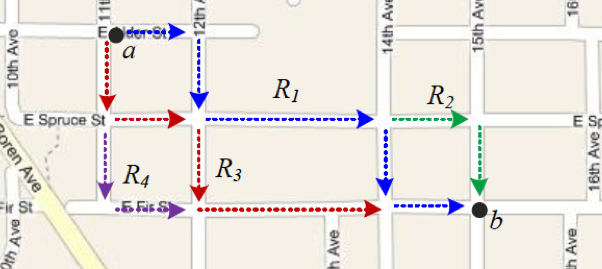
\includegraphics{low_sample_rate}
\centering
\caption{Example of low sample rate problem}
\end{figure}

\subsection{Post Multiply Normalization}

When more than two multiplications are performed in a row, the intermediate
normalization of the results between multiplications can be eliminated.
This is because with each multiplication, the mantissa can become
denormalized by at most one bit.  If there are guard bits on the mantissas
to prevent bits from ``falling off'' the end during multiplications, the
normalization can be postponed until after a sequence of several
multiplies\footnote{Using unnormalized numbers for math is not a new idea; a
good example of it is the Control Data CDC 6600, designed by Seymour Cray.
\cite{thornton:cdc6600} The CDC 6600 had all of its instructions performing
unnormalized arithmetic, with a separate {\tt NORMALIZE} instruction.}.

% This is an example of how you would use tgrind to include an example
% of source code; it is commented out in this template since the code
% example file does not exist.  To use it, you need to remove the '%' on the
% beginning of the line, and insert your own information in the call.
%
%\tagrind[htbp]{code/pmn.s.tex}{Post Multiply Normalization}{opt:pmn}

As you can see, the intermediate results can be multiplied together, with no
need for intermediate normalizations due to the guard bit.  It is only at
the end of the operation that the normalization must be performed, in order
to get it into a format suitable for storing in memory\footnote{Note that
for purposed of clarity, the pipeline delays were considered to be 0, and
the branches were not delayed.}.

\subsection{Block Exponent}

In a unoptimized sequence of additions, the sequence of operations is as
follows for each pair of numbers ($m_1$,$e_1$) and ($m_2$,$e_2$).
\begin{enumerate}
  \item Compare $e_1$ and $e_2$.
  \item Shift the mantissa associated with the smaller exponent $|e_1-e_2|$
        places to the right.
  \item Add $m_1$ and $m_2$.
  \item Find the first one in the resulting mantissa.
  \item Shift the resulting mantissa so that normalized
  \item Adjust the exponent accordingly.
\end{enumerate}

Out of 6 steps, only one is the actual addition, and the rest are involved
in aligning the mantissas prior to the add, and then normalizing the result
afterward.  In the block exponent optimization, the largest mantissa is
found to start with, and all the mantissa's shifted before any additions
take place.  Once the mantissas have been shifted, the additions can take
place one after another\footnote{This requires that for n consecutive
additions, there are $\log_{2}n$ high guard bits to prevent overflow.  In
the $\mu$FPU, there are 3 guard bits, making up to 8 consecutive additions
possible.}.  An example of the Block Exponent optimization on the expression
X = A + B + C is given in figure~\ref{opt:be}.

% This is an example of how you would use tgrind to include an example
% of source code; it is commented out in this template since the code
% example file does not exist.  To use it, you need to remove the '%' on the
% beginning of the line, and insert your own information in the call.
%
%\tgrind[htbp]{code/be.s.tex}{Block Exponent}{opt:be}

\section{Integer optimizations}

As well as the floating point optimizations described above, there are
also integer optimizations that can be used in the $\mu$FPU.  In concert
with the floating point optimizations, these can provide a significant
speedup.  

\subsection{Conversion to fixed point}

Integer operations are much faster than floating point operations; if it is
possible to replace floating point operations with fixed point operations,
this would provide a significant increase in speed.

This conversion can either take place automatically or or based on a
specific request from the programmer.  To do this automatically, the
compiler must either be very smart, or play fast and loose with the accuracy
and precision of the programmer's variables.  To be ``smart'', the computer
must track the ranges of all the floating point variables through the
program, and then see if there are any potential candidates for conversion
to floating point.  This technique is discussed further in
section~\ref{range-tracking}, where it was implemented.

The other way to do this is to rely on specific hints from the programmer
that a certain value will only assume a specific range, and that only a
specific precision is desired.  This is somewhat more taxing on the
programmer, in that he has to know the ranges that his values will take at
declaration time (something normally abstracted away), but it does provide
the opportunity for fine-tuning already working code.

Potential applications of this would be simulation programs, where the
variable represents some physical quantity; the constraints of the physical
system may provide bounds on the range the variable can take.
\subsection{Small Constant Multiplications}

One other class of optimizations that can be done is to replace
multiplications by small integer constants into some combination of
additions and shifts.  Addition and shifting can be significantly faster
than multiplication.  This is done by using some combination of
\begin{eqnarray*}
a_i & = & a_j + a_k \\
a_i & = & 2a_j + a_k \\
a_i & = & 4a_j + a_k \\
a_i & = & 8a_j + a_k \\
a_i & = & a_j - a_k \\
a_i & = & a_j \ll m \mbox{shift}
\end{eqnarray*}
instead of the multiplication.  For example, to multiply $s$ by 10 and store
the result in $r$, you could use:
\begin{eqnarray*}
r & = & 4s + s\\
r & = & r + r
\end{eqnarray*}
Or by 59:
\begin{eqnarray*}
t & = & 2s + s \\
r & = & 2t + s \\
r & = & 8r + t
\end{eqnarray*}
Similar combinations can be found for almost all of the smaller
integers\footnote{This optimization is only an ``optimization'', of course,
when the amount of time spent on the shifts and adds is less than the time
that would be spent doing the multiplication.  Since the time costs of these
operations are known to the compiler in order for it to do scheduling, it is
easy for the compiler to determine when this optimization is worth using.}.
\cite{magenheimer:precision}

\section{Other optimizations}

\subsection{Low-level parallelism}

The current trend is towards duplicating hardware at the lowest level to
provide parallelism\footnote{This can been seen in the i860; floating point
additions and multiplications can proceed at the same time, and the RISC
core be moving data in and out of the floating point registers and providing
flow control at the same time the floating point units are active. \cite{byte:i860}}

Conceptually, it is easy to take advantage to low-level parallelism in the
instruction stream by simply adding more functional units to the $\mu$FPU,
widening the instruction word to control them, and then scheduling as many
operations to take place at one time as possible.

However, simply adding more functional units can only be done so many times;
there is only a limited amount of parallelism directly available in the
instruction stream, and without it, much of the extra resources will go to
waste.  One process used to make more instructions potentially schedulable
at any given time is ``trace scheduling''.  This technique originated in the
Bulldog compiler for the original VLIW machine, the ELI-512.
\cite{ellis:bulldog,colwell:vliw}  In trace scheduling, code can be
scheduled through many basic blocks at one time, following a single
potential ``trace'' of program execution.  In this way, instructions that
{\em might\/} be executed depending on a conditional branch further down in
the instruction stream are scheduled, allowing an increase in the potential
parallelism.  To account for the cases where the expected branch wasn't
taken, correction code is inserted after the branches to undo the effects of
any prematurely executed instructions.

\subsection{Pipeline optimizations}

In addition to having operations going on in parallel across functional
units, it is also typical to have several operations in various stages of
completion in each unit.  This pipelining allows the throughput of the
functional units to be increased, with no increase in latency.

There are several ways pipelined operations can be optimized.  On the
hardware side, support can be added to allow data to be recirculated back
into the beginning of the pipeline from the end, saving a trip through the
registers.  On the software side, the compiler can utilize several tricks to
try to fill up as many of the pipeline delay slots as possible, as
seendescribed by Gibbons. \cite{gib86}


